\documentclass[10pt]{article}
\usepackage[margin=0.9in]{geometry}
\usepackage[T1]{fontenc}
\usepackage{times}
\usepackage{amsmath}
\usepackage{graphicx}
\usepackage{booktabs}
\usepackage{microtype}
\usepackage[numbers]{natbib}
\setlength{\bibsep}{0pt}
\usepackage[dvipsnames]{xcolor}
\usepackage[colorlinks=true,linkcolor=blue!50!black,citecolor=blue!50!black,urlcolor=blue!50!black]{hyperref}
\usepackage{caption}
\captionsetup{font=small,labelfont=bf}
\usepackage{subcaption}
\captionsetup[subfigure]{labelformat=empty,justification=raggedright,singlelinecheck=false}
\setlength{\parskip}{2pt}
\setlength{\parindent}{0pt}

\title{\vspace{-0.6em}\textbf{Sampling Better Neural Cellular Automata for Pretraining}\vspace{-0.2em}}
\author{Sagnik Bhattacharjee\\
\href{mailto:sbcharjee.acad@gmail.com}{sbcharjee.acad@gmail.com}\quad
\href{https://x.com/datavorous_}{@datavorous\_}}
\date{\textit{Draft}}

\begin{document}
\maketitle
\vspace{-1.2em}

\begin{abstract}
\noindent Pre-pretraining language models on neural cellular automata (NCA) trajectories can speed up later language training. We ask whether choosing which NCA worlds to train on matters beyond filtering them by gzip complexity. Using a 1M parameter Transformer on TinyStories, we reproduce the NCA transfer benefit and find that most of it remains after shuffling the NCA tokens. We then test several simple properties of NCA trajectories and find that worlds with higher horizontal recurrence transfer better, while selecting for lower recurrence hurts. A stronger recurrence filter reduces the downstream tokens needed to reach the same validation loss by about 17\% compared with ordinary NCA.
\end{abstract}

\section{Introduction}

Lee et al.\ \citep{lee2026nca} show that language models can benefit from pre-pretraining on trajectories generated by neural cellular automata (NCA) before seeing natural language. They report faster downstream convergence and lower language modeling loss, and find that the best NCA complexity depends on the target domain. Their main control for choosing trajectories is gzip compressibility \citep{deutsch1996gzip}.

Compressibility is useful, but coarse. Two trajectories can have similar gzip complexity while exposing a Transformer to very different local structure. We therefore ask a narrower question: among NCA trajectories with similar complexity, are some better pretraining data than others?

We study this at small scale with a 1M parameter Transformer. We keep the NCA generator, token budget, gzip range, and model fixed, and change only which trajectories are selected for pretraining. We first reproduce the NCA transfer effect, then test whether simple properties of the generated trajectories predict better downstream learning.

\section{Setup}

\paragraph{NCA data}
We follow the NCA generation and tokenization setup of Lee et al.\ \citep{lee2026nca}. Each world is a $12{\times}12$ grid with 10 cell states. We first let each NCA evolve for 10 steps. We record 27 frames and split each into nonoverlapping $2\times2$ patches. Each frame contains 36 patches and two frame markers, giving 1,026 tokens per world. We group trajectories into four gzip complexity bands: $[.2,.3)$, $[.3,.4)$, $[.4,.5)$, and $[.5,\infty)$. Each NCA pretraining run uses 19.7M scored tokens.

\paragraph{Model and transfer}
We use a small causal Transformer \citep{vaswani2017attention} with 4 layers, 2 attention heads, width 20, and context length 256. It has 1.08M parameters with the language vocabulary. After NCA pretraining, we discard the NCA embeddings and output head, transfer the Transformer body, and initialize a new language embedding and tied output head. We then train on 10M TinyStories tokens \citep{eldan2023tinystories}. All paired conditions use the same data order, optimization schedule, and model initialization. We evaluate five model seeds unless stated otherwise.

\paragraph{Evaluation}
Our primary measurement is validation loss at fixed TinyStories token counts. We also report downstream sample efficiency as the number of language tokens needed to reach the loss obtained by the corresponding scratch model after 10M tokens. Crossings between evaluation checkpoints are linearly interpolated. This metric counts language tokens only and does not include the cost of NCA pretraining.


\section{Results}

\subsection{Shuffling Preserves Transfer}

All four NCA bands outperform Scratch (language training without NCA pretraining) at 10M TinyStories tokens (Fig.~\ref{fig:curves}, Table~\ref{tab:main}). The 40-50\% gzip band performs best on average, with validation loss $4.185\pm0.024$ compared with $4.322\pm0.020$ for Scratch. This corresponds to a downstream-token speedup of $1.77\pm0.21\times$.

We use Ordinary NCA (unfiltered worlds from the 40--50\% gzip band) as the reference condition for later experiments.

The differences between the middle gzip bands are small. The 40-50\% band is only 0.010 lower in loss than the 30-40\% band, and it has the best final loss in 2/5 seeds. We therefore do not find a clear optimal gzip band.

The NCA advantage is largest early in language training. At 0.5M tokens, the gap to scratch is about 1.08 loss. By 10M tokens, it has narrowed to roughly 0.09-0.14.

We then shuffle the patch tokens inside each NCA trajectory while keeping the same tokens. The shuffled control reaches $4.203\pm0.025$ validation loss. The best structured band is only 0.018 lower. Most of the NCA transfer benefit therefore survives shuffling.

\begin{figure}[!htbp]
\centering
\begin{subfigure}[t]{0.49\textwidth}
\centering
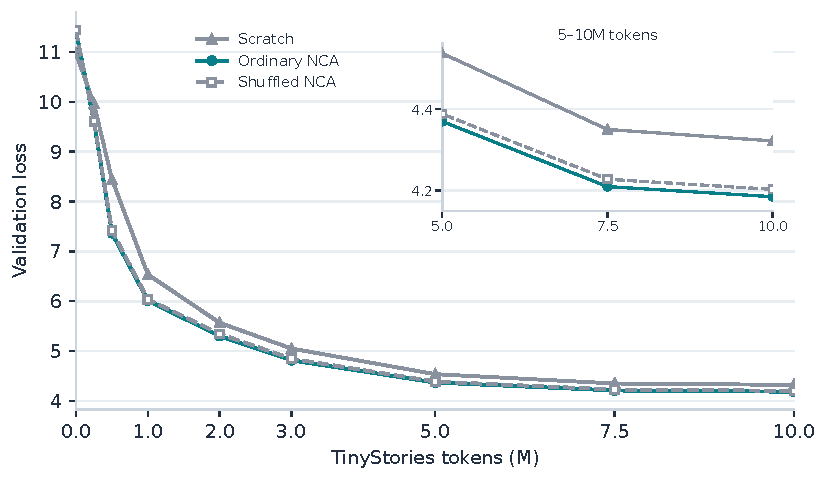
\includegraphics[width=\linewidth]{figs_cool/fig1_reproduction_curves.pdf}
\caption{TinyStories validation loss for Scratch, shuffled NCA, and ordinary NCA, averaged over five seeds. The inset shows the final 5M tokens.}
\end{subfigure}\hfill
\begin{subfigure}[t]{0.49\textwidth}
\centering
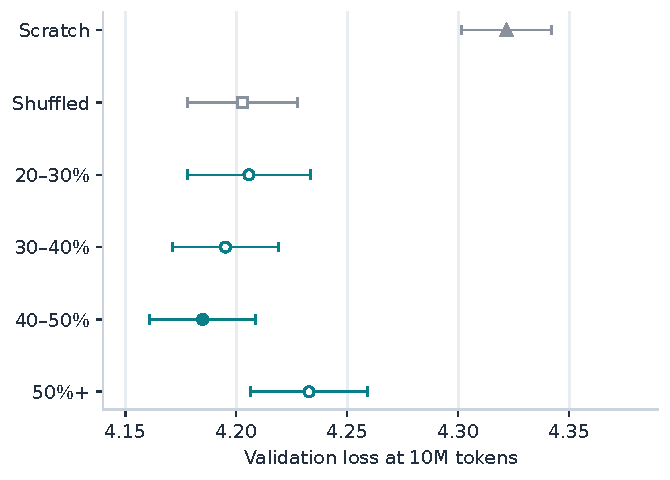
\includegraphics[width=\linewidth]{figs_cool/fig1_reproduction_bands.pdf}
\caption{Final validation loss for Scratch, shuffled NCA, and four gzip bands. Points show seed means; whiskers show one standard deviation.}
\end{subfigure}
\caption{NCA pretraining improves over Scratch, while differences between gzip bands remain small.}
\label{fig:curves}
\end{figure}

\begin{table}[!htbp]
\centering\small
\caption{Validation loss after 10M TinyStories tokens. Speedup measures how quickly each condition reaches the final loss of its paired scratch model.}
\label{tab:main}
\begin{tabular}{lcccc}
\toprule
Condition & Val.\ loss & PPL & Gain vs.\ scratch & Speedup \\
\midrule
Scratch & $4.322\pm0.020$ & 75.33 & -- & $1.00\times$ \\
Shuffled NCA & $4.203\pm0.025$ & 66.88 & $0.119\pm0.043$ & $1.68\pm0.21\times$ \\
20-30\% gzip & $4.206\pm0.028$ & 67.09 & $0.116\pm0.041$ & $1.64\pm0.21\times$ \\
30-40\% gzip & $4.195\pm0.024$ & 66.38 & $0.127\pm0.009$ & $1.70\pm0.06\times$ \\
40-50\% gzip & $4.185\pm0.024$ & 65.70 & $0.137\pm0.039$ & $1.77\pm0.21\times$ \\
50\%+ gzip & $4.233\pm0.026$ & 68.93 & $0.089\pm0.039$ & $1.56\pm0.15\times$ \\
\bottomrule
\end{tabular}
\end{table}


\subsection{Recurrence Helps}

We next ask whether simple properties of an NCA trajectory can predict better transfer. We test six ways of selecting worlds within the 40-50\% gzip band. Changes in cell activity, spatial agreement, and transition mutual information do not improve downstream learning.

One property does. Some worlds repeat horizontally adjacent $2\times2$ patches more often than expected from their overall patch frequencies.

We call this horizontal recurrence. It gives each world a recurrence score that can be computed before language model training. Each frame contains $6\times6=36$ nonoverlapping patches and $6\times5=30$ horizontal patch pairs, giving $N=27\times36=972$ patches and 810 horizontal pairs per world. Let $p_{t,r,c}$ denote the patch ID at frame $t$, row $r$, and column $c$, and let $n_v$ be the number of occurrences of patch ID $v$.

\[
R_h =
\frac{1}{810}
\sum_{t=1}^{27}
\sum_{r=1}^{6}
\sum_{c=2}^{6}
\mathbf{1}[p_{t,r,c}=p_{t,r,c-1}]
-
\frac{\sum_v n_v(n_v-1)}{N(N-1)}.
\]

The first term measures how often horizontally neighboring patches match. The second subtracts the match rate expected from the same patch counts under random ordering.

Selecting worlds with higher horizontal recurrence improves the loss after 1M TinyStories tokens by $0.059\pm0.030$ across five seeds. Selecting worlds with lower recurrence makes it worse by $0.043\pm0.015$.

We first found this pattern on one corpus, so we repeated the experiment on three new sets of NCA rules. Each set contains high recurrence, ordinary, and low recurrence worlds, evaluated with five model seeds. High recurrence beats ordinary NCA in 14/15 paired runs, and its average effect is positive in all three rule populations. Ordinary NCA beats low recurrence in 12/15 runs (Fig.~\ref{fig:selection}).

Across the three new rule populations, high recurrence improves the 1M token loss by $0.053\pm0.006$ on average. Since these three populations are the independent replications, we treat this as consistent directional evidence rather than statistical significance.

\begin{figure}[!htbp]
\centering
\begin{subfigure}[t]{0.49\textwidth}
\centering
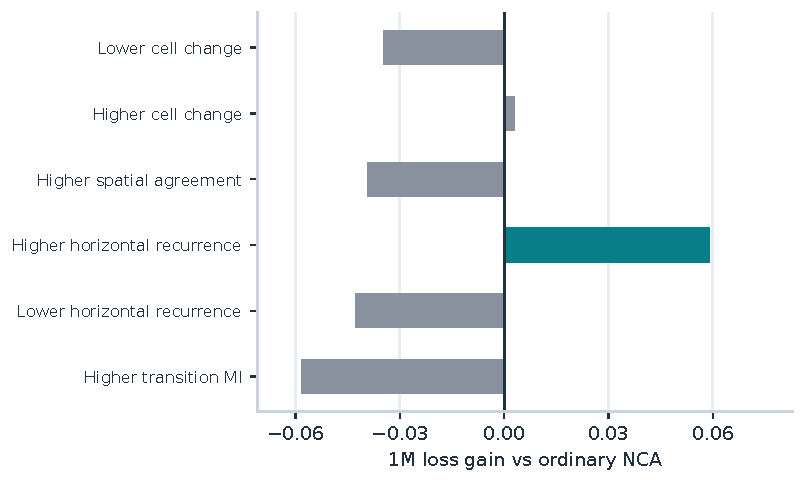
\includegraphics[width=\linewidth]{figs_cool/fig2_recurrence_selectors.pdf}
\caption{Effects of trajectory selectors after 1M TinyStories tokens. Positive values mean lower loss than ordinary NCA.}
\end{subfigure}\hfill
\begin{subfigure}[t]{0.49\textwidth}
\centering
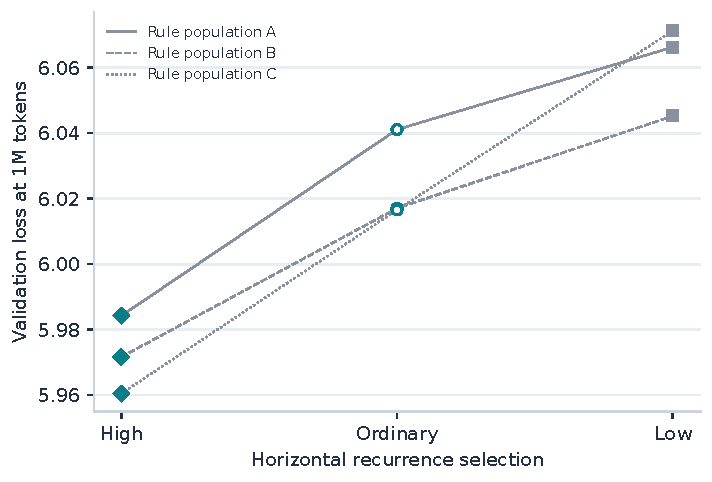
\includegraphics[width=\linewidth]{figs_cool/fig2_recurrence_replicates.pdf}
\caption{Mean validation loss for high recurrence, ordinary NCA, and low recurrence across three independent rule populations. Lower is better.}
\end{subfigure}
\caption{Trajectory selection across independently generated NCA corpora.}
\label{fig:selection}
\end{figure}

\paragraph{What does recurrence capture?}
Horizontal patch recurrence is strongly related to other properties of the NCA dynamics, including lag-2 recurrence and transition mutual information. These features move together under our selector. We therefore treat recurrence as a useful way to select worlds, not as an isolated causal mechanism.

\subsection{Stronger Selection}

We next strengthen the recurrence filter. We choose its cutoff on the discovery data and freeze it before the confirmation experiment.

We test the stronger filter on three independently generated NCA corpora. For each corpus, Ordinary and Designed (top 10\% by horizontal recurrence) use the same gzip distribution and NCA token budget. We train both conditions with five model initializations.

\begin{table}[!htbp]
\centering\small
\caption{Results after 10M TinyStories tokens.}
\label{tab:stronger-selection}
\begin{tabular}{lccccc}
\toprule
Condition & Val.\ loss & PPL & Gain vs.\ scratch & Gain vs.\ Ordinary & Speedup\\
\midrule
Scratch & $4.322\pm0.020$ & 75.33 & -- & -- & $1.000\times$\\
Ordinary NCA & $4.199\pm0.007$ & 66.64 & 0.123 & -- & $1.647\pm0.045\times$\\
Designed NCA & $4.149\pm0.007$ & 63.39 & 0.173 & $0.050\pm0.014$ & $1.983\pm0.041\times$\\
\bottomrule
\end{tabular}
\end{table}


Across the three corpora, Designed outperforms Ordinary. At 10M TinyStories tokens, it lowers validation loss by $0.050\pm0.014$ on average across the three corpus means (Table~\ref{tab:stronger-selection}).

The same pattern appears in convergence speed. Ordinary reaches the paired Scratch endpoint with a mean speedup of $1.647\pm0.045\times$, while Designed reaches it at $1.983\pm0.041\times$. This corresponds to about 6.07M TinyStories tokens for Ordinary and 5.04M for Designed, or about 17\% fewer downstream tokens.

The advantage appears early in training (Fig.~\ref{fig:confirmation}). The mean validation loss improvement peaks at about 0.15 near 2M TinyStories tokens, then gradually narrows. It remains positive through 10M tokens.

\begin{figure}[!htbp]
\centering
\begin{subfigure}[t]{0.49\textwidth}
\centering
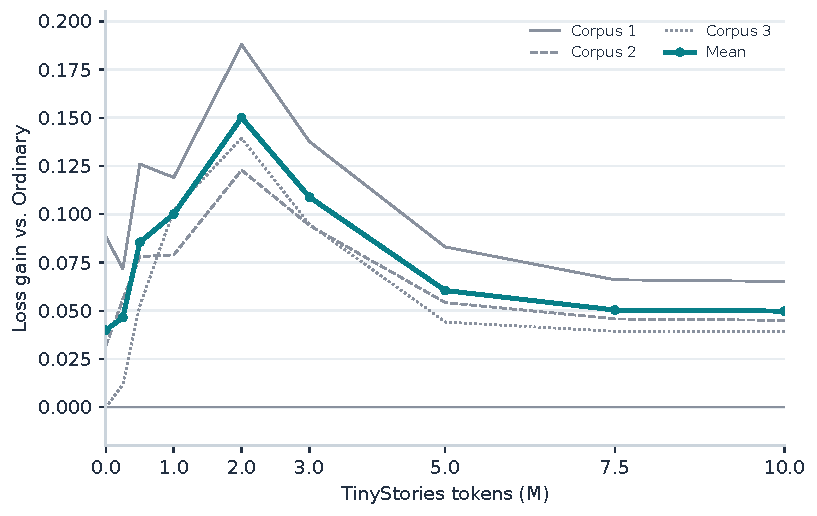
\includegraphics[width=\linewidth]{figs_cool/fig3_confirmation_loss.pdf}
\caption{Designed gain over Ordinary during training. Thin lines show corpus means; the green line shows their overall mean.}
\end{subfigure}\hfill
\begin{subfigure}[t]{0.49\textwidth}
\centering
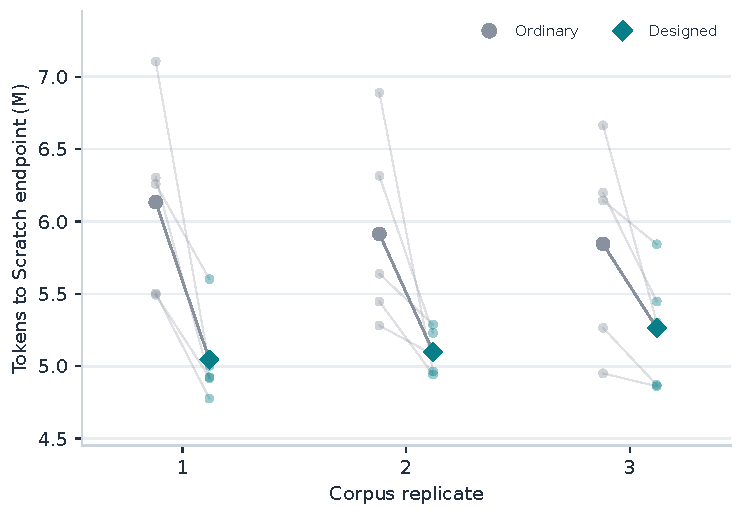
\includegraphics[width=\linewidth]{figs_cool/fig3_confirmation_tokens.pdf}
\caption{Tokens to the paired Scratch endpoint. Small points show model runs; large points show corpus means. Fewer is better.}
\end{subfigure}
\caption{Effect of stronger recurrence selection.}
\label{fig:confirmation}
\end{figure}


\section{Related Work}

Language models can benefit from training on structured data that is not natural language \citep{shinnick2025procedural}. Prior work has explored music \citep{papadimitriou2020music}, synthetic tasks \citep{wu2022insights}, and formal languages \citep{hu2025circuits} as sources of useful pretraining structure.

Lee et al.\ \citep{lee2026nca} extend this idea to trajectories generated by neural cellular automata \citep{mordvintsev2020growing}. They show that NCA pre-pretraining can improve later language training \citep{yamaguchi2026synthetic}, and that the best NCA complexity depends on the downstream domain. We follow their released generation and tokenization setup.

\section{Limitations}

We study only a 1M parameter Transformer on TinyStories and use one NCA generator. Whether the same selection strategy helps larger models or other downstream datasets remains open.

The recurrence score is also not an isolated mechanism. Worlds with more horizontal recurrence differ in other ways, including lag-2 recurrence and transition mutual information. Our experiments therefore show that recurrence is useful for selecting NCA worlds, not that patch repetition itself causes better transfer.

Finally, our speedup metric counts only downstream language tokens and estimates crossings between evaluation checkpoints. We therefore treat it as a summary of learning speed rather than total training efficiency.

\section{Conclusion}

In our experiments, we found that the choice of NCA worlds matters. Selecting trajectories with more horizontal recurrence improves downstream language learning beyond gzip based filtering. The same direction appears across newly generated rule populations.

More broadly, our results suggest that NCA sampling itself can be hill-climbed. The space of generated worlds contains useful structure, and simple selection rules can move the training distribution toward worlds that transfer better.

\bibliographystyle{plainnat}
\renewcommand{\bibfont}{\small}
\bibliography{references}
\end{document}
